\section{Deployment view}

I dette afsnit beskrives hvilke softwareklasser der bruges i systemets mest grundlæggende moduler. Desuden beskrives hvilke protokoller der anvendes mellem de grundlæggende moduler i systemet, fx. beskrives layout af meddelelser der sendes mellem drone og server.


\begin{figure}[H]
\centering
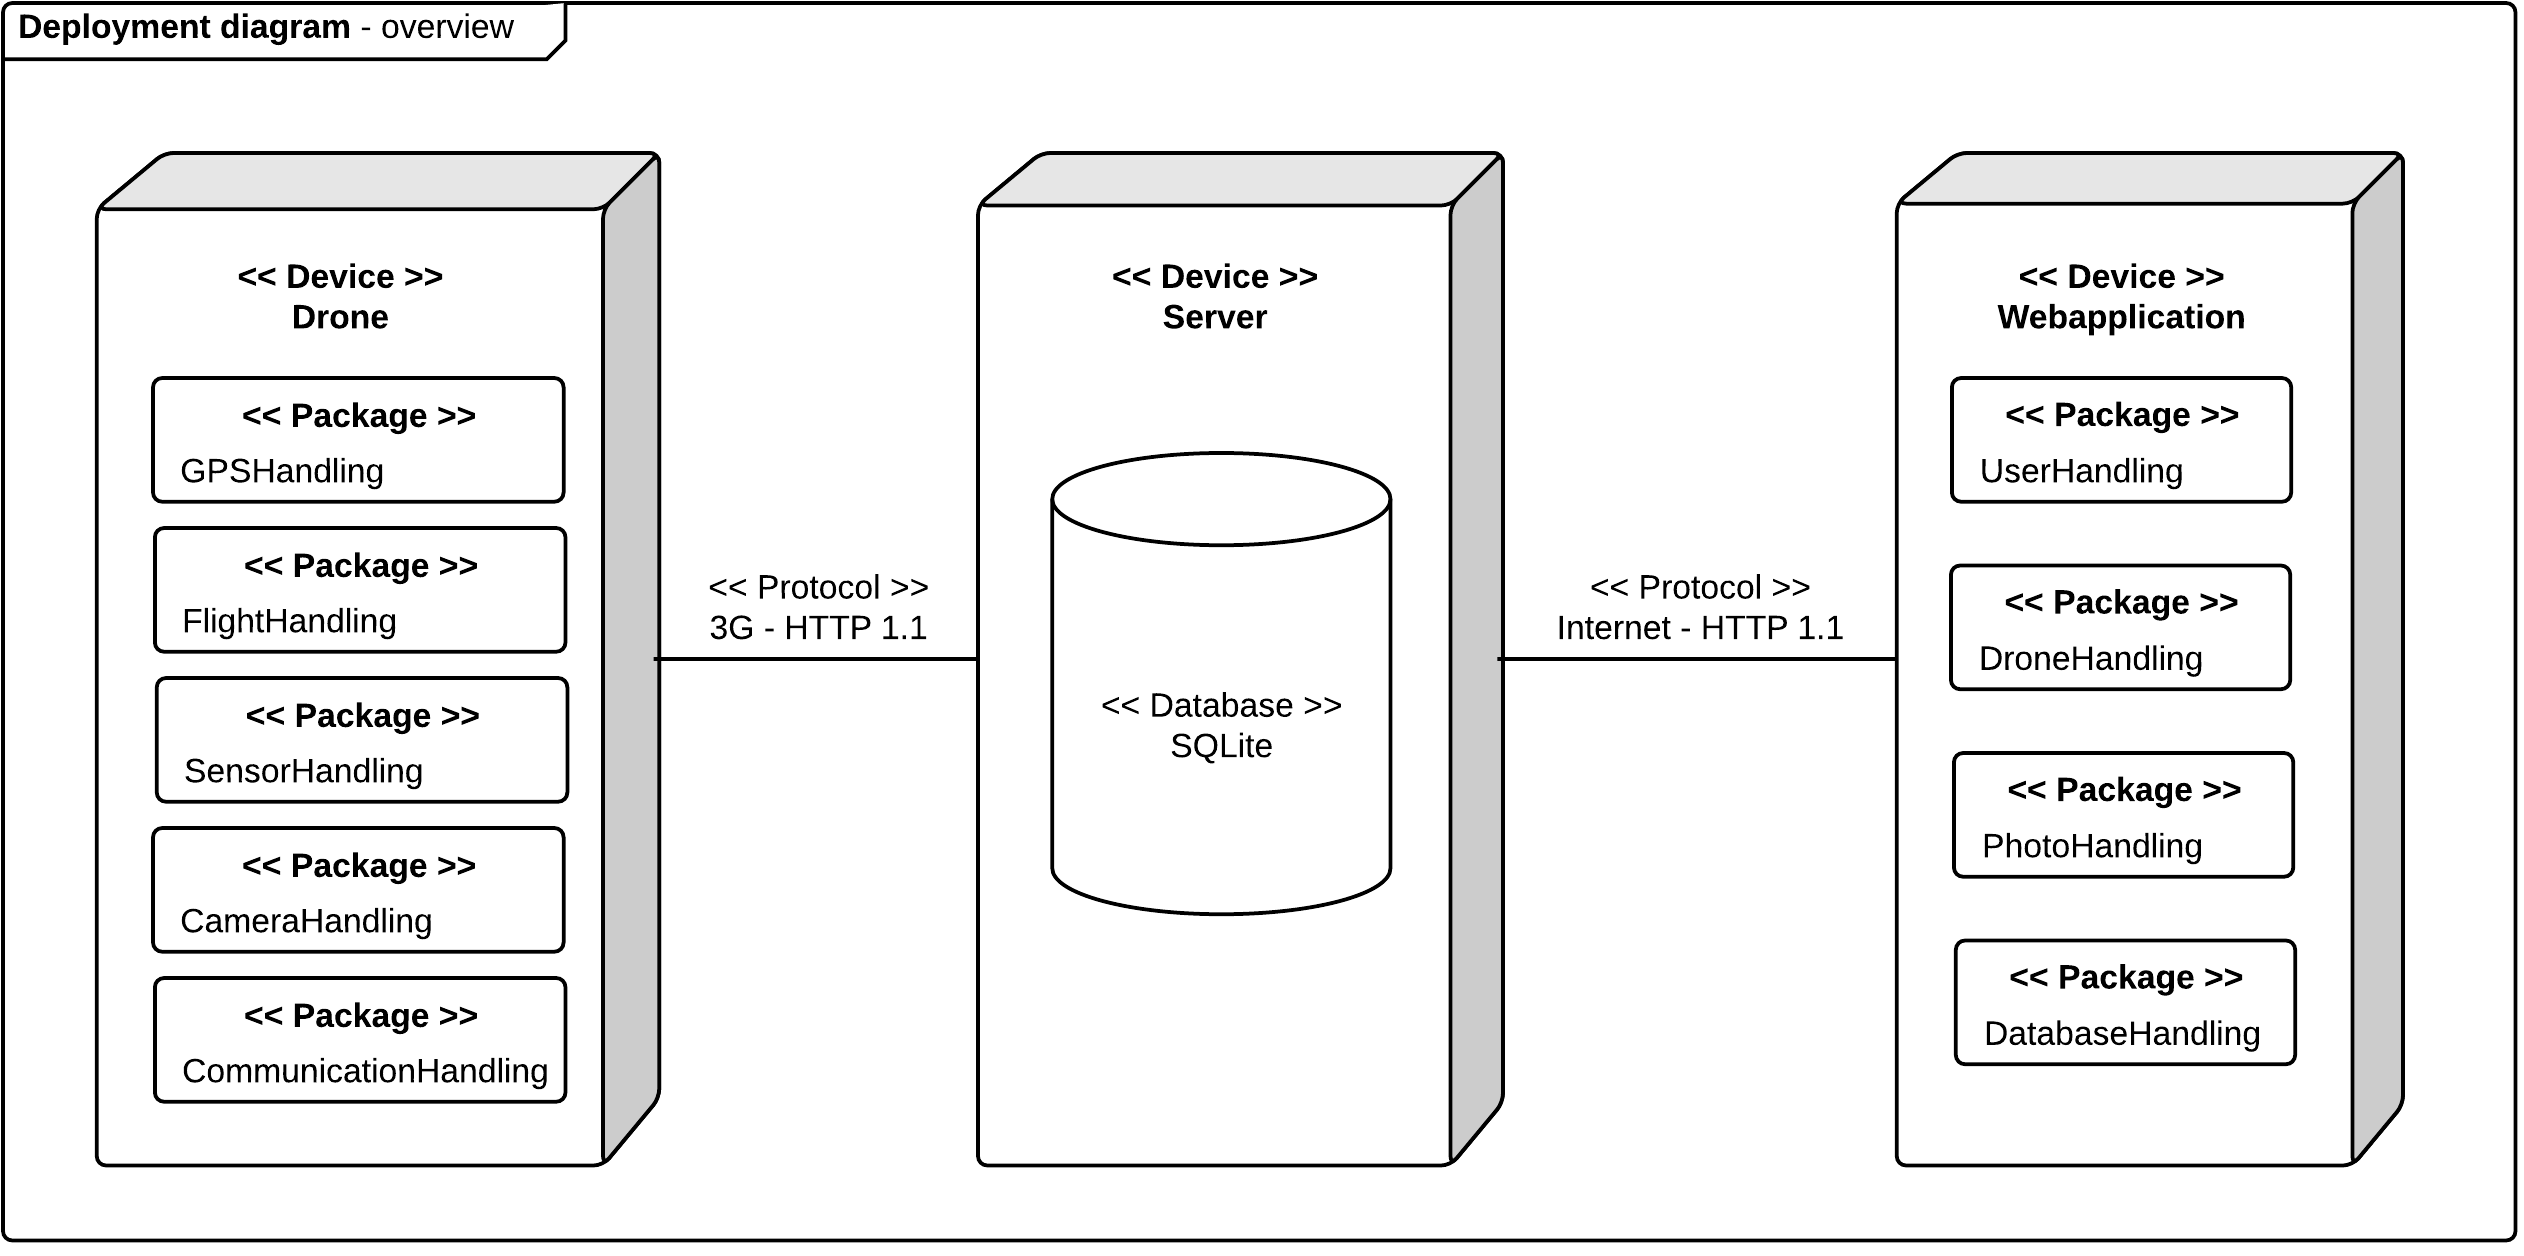
\includegraphics[width=1\textwidth]{Billeder/deployment_overview.png}
\caption{Overordnet deployment diagram}
\label{fig:deployment_generel}
\end{figure}


På illustrationen figur \ref{fig:deployment_generel} vises systemet opdelt i de 3 mest grundlæggende moduler. Som det ses af illustrationen består systemet overordnet set af drone, webapplikation og sever. I de følgende afsnit vil de tre overordnede moduler blive pakket op og forklaret hver for sig, og desuden vil HTTP 1.1 protokollen blive beskrevet.



\newpage
\subsection{HTTP 1.1 protokol}

For at kunne udveklse informationer mellem server og drone er der blevet anvendt en protokol. Protokollen er blevet valgt på baggrund af kommunikations måden, men også ifht. kommunikationen mellem websitet og serveren. Websitet kommer til at kommunikere med serveren på samme måde som dronen vil, derfor er det passende at bruge samme protokol. 
Valget blev at anvende HTTP protokollen. HTTP er en protokol der befinder sig i applikations laget, som er det øverste lag i internet protokollen. Det er dette lag der håndterer kommunikationen eller udveksling af data over internettet. 
Clienten (I dette tilfælde dronen) laver et request til serverens URL ved at oprette en TCP forbindelse. Når denne forbindelse er oprettet, kan clienten kalde http requesten i form af forskellige kommandoer. De forskellige kommandoer kan beskrives som CRUD (Create, Read, Update \& Delete) metoder. 
Med disse kommandoer vil dronen være i stand til at kommunikere og få de information der er nødvendige for at kunne flyve til de forskellige koordinater.

Dronen anvender HTTP 1.1, da der er flere metoder at gøre brug af. 
Dronen bruger 3 metoder til at kommunikere med serveren: GET, POST \& PUT. 
\begin{itemize}
	\item GET: henter data fra serveren.
	\item POST: Sender data til serveren, hvor serveren så opretter objektet.
	\item PUT: Opdaterer data på serveren og hvis der ikke allerede findes den type data, opretter serveren objektet.
\end{itemize}

Når clienten laver en get request, vil serveren svare med en header og body. Headeren vil indeholde en status besked. Denne status besked fortæller om requesten er gået igennem eller om der er sket en fejl undervejs.Ved en succesfuld modtagelse, vil der stå http 200 OK. Udover status beskeden vil header også bestå af meta data, som fx. hvilket format beskeden er i. 
Bodyen der modtages indeholder således de ønskede data fra serveren.

Ved et post eller put request, skal dronen sende en header fil samt en body med de data der ønskes udvekslet til serveren. 
Ved put er det vigtigt at det data der ønskes sendt har samme format som det der ligger på serveren, ellers melder status beskeden at der er en fejl. 




% http://en.wikipedia.org/wiki/Hypertext_Transfer_Protocol
